% The CNN bit decoder in codes/cnn_decoder.py, drawn with PlotNeuralNet's TikZ layers
% (layers/, MIT licence, https://github.com/HarisIqbal88/PlotNeuralNet).
% Build with: python3 -m experiments.plot_network_latex
%
% Each block is one tensor: thickness = channels, height and depth fixed,
% the receding axis = time (80 envelope steps = 5 bits x 16 steps).
\documentclass[border=15pt, multi, tikz]{standalone}
\usepackage{import}
\subimport{layers/}{init}
\usetikzlibrary{positioning}
\usetikzlibrary{3d}
\usetikzlibrary{calc}
\newcommand{\under}[2]{\node[anchor=north, align=center, font=\small] at ($($(#1-nearsouthwest)!0.5!(#1-nearsoutheast)$)+(0,-1.35cm)$) {#2};}

\def\InputColor{rgb:blue,2;green,1;white,6}
\def\ConvColor{rgb:yellow,5;red,2.5;white,5}
\def\ConvReluColor{rgb:yellow,5;red,5;white,5}
\def\DenseColor{rgb:blue,2;red,3;white,8}
\def\OutColor{rgb:red,5;yellow,1;black,1}
\def\AuxColor{rgb:blue,5;green,2.5;white,5}

\begin{document}
\begin{tikzpicture}
\tikzstyle{connection}=[ultra thick,every node/.style={sloped,allow upside down},draw=\edgecolor,opacity=0.7]

%% (zy canvas mirrors images, so \reflectbox puts the text the right way round)
%% Input: the envelope of the bit being decided and 2 bits either side (real recording)
\node[canvas is zy plane at x=0] (env) at (-5.2,0,0) {\reflectbox{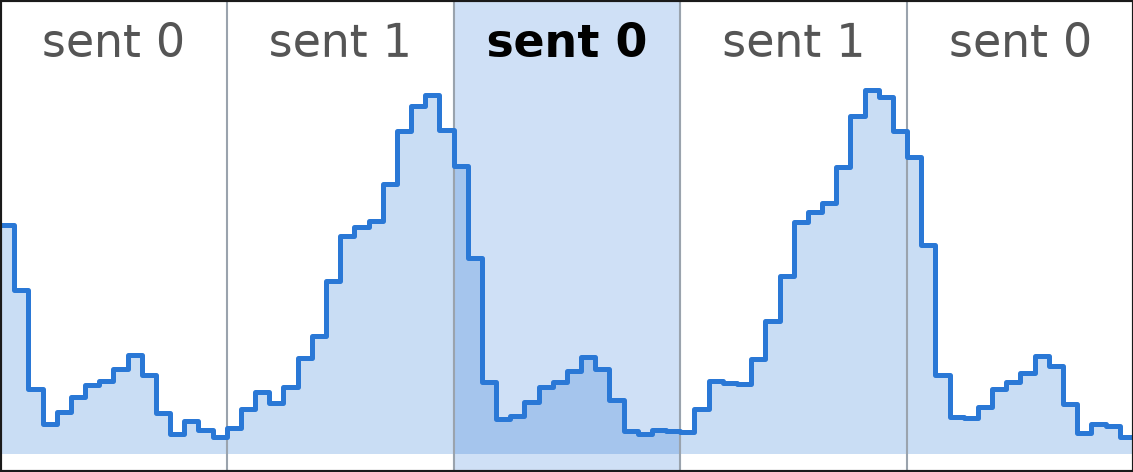
\includegraphics[width=9.6cm,height=4cm]{envelope_input.png}}};
\node[anchor=north, align=center] at (-5.2,-3.6,0) {\bf envelope\\[-1pt]\small 5 bits $\times$ 16 steps};

%% Input tensor: envelope, log envelope, 'bit exists' flag
\pic[shift={(0,0,0)}] at (0,0,0) {Box={name=inp,caption=input,%
        xlabel={{"","3",""}},zlabel=80,fill=\InputColor,opacity=0.6,%
        height=20,width={1,1,1},depth=48}};

%% conv1, conv2: 16 filters of width 5, ReLU
\pic[shift={(2.6,0,0)}] at (inp-east) {RightBandedBox={name=c1,caption=conv1,%
        xlabel={{"16",""}},zlabel=80,fill=\ConvColor,bandfill=\ConvReluColor,%
        height=20,width=4,depth=48}};
\pic[shift={(2.6,0,0)}] at (c1-east) {RightBandedBox={name=c2,caption=conv2,%
        xlabel={{"16",""}},zlabel=80,fill=\ConvColor,bandfill=\ConvReluColor,%
        height=20,width=4,depth=48}};

%% flatten (dropout 0.3), dense 32 + ReLU
\pic[shift={(2.4,0,0)}] at (c2-east) {Box={name=fl,caption=flatten,%
        xlabel={{"1280",""}},fill=\ConvColor,opacity=0.6,%
        height=36,width=1,depth=3}};
\pic[shift={(1.6,0,0)}] at (fl-east) {RightBandedBox={name=fc,caption=dense,%
        xlabel={{"32",""}},fill=\DenseColor,bandfill=\ConvReluColor,%
        height=11,width=1.4,depth=3}};

%% Two heads
\pic[shift={(2.4,2.2,0)}] at (fc-east) {Box={name=pb,%
        xlabel={{"1",""}},fill=\OutColor,opacity=0.75,%
        height=4,width=1.2,depth=4}};
\pic[shift={(2.4,-2.2,0)}] at (fc-east) {Box={name=tr,%
        xlabel={{"4",""}},fill=\AuxColor,opacity=0.75,%
        height=4,width=2.4,depth=4}};
\node[anchor=west, align=left] at ([xshift=0.5cm]pb-east) {\bf $P(\mathrm{bit}=1)$\\\small $\geq 0.5 \rightarrow 1$};
\node[anchor=west, align=left] at ([xshift=0.5cm]tr-east) {\bf transition\\\small training only};

%% Notes under the blocks
\under{inp}{envelope, log envelope,\\ `bit exists' flag}
\under{c1}{width 5, ReLU}
\under{c2}{width 5, ReLU}
\under{fl}{dropout 0.3}
\under{fc}{ReLU}

%% Connections
\draw [connection] ([xshift=-3.2cm]inp-west) -- node {\midarrow} (inp-west);
\draw [connection] (inp-east) -- node {\midarrow} (c1-west);
\draw [connection] (c1-east)  -- node {\midarrow} (c2-west);
\draw [connection] (c2-east)  -- node {\midarrow} (fl-west);
\draw [connection] (fl-east)  -- node {\midarrow} (fc-west);
\path (fc-east) -- (pb-west|-fc-east) coordinate[pos=0.45] (split);
\draw [connection] (fc-east) -- (split) -- (split|-pb-west) -- node {\midarrow} (pb-west);
\draw [connection] (split) -- (split|-tr-west) -- node {\midarrow} (tr-west);

%% Title and key
\node[anchor=south, font=\Large\bfseries] at ([yshift=1.9cm]c2-north) {Network bit decoder ($\approx$ 43,000 parameters)};
\node[anchor=north, font=\small, text=black!65] at ([yshift=-4.4cm]c2-south)
     {block thickness = channels \quad$\cdot$\quad receding axis = time (80 steps = 5 bits) \quad$\cdot$\quad dark band = ReLU};

\end{tikzpicture}
\end{document}
